% Number 560
% UFPM  Algebra Units CAPMA 
% Airbag Stop
% KO/JG

% Watermark
\AddToShipoutPicture*{\BackgroundPic}

\addtocounter {ProbNum} {1}

%\begin{floatingfigure}[r]{.2\textwidth}
%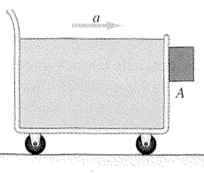
\includegraphics[scale=.6]{/Users/jgates/desktop/latex/pics/cartstatic}
%\end{floatingfigure}
 
{\bf \Large{\arabic{ProbNum}}} The human body can survive a negative acceleration trauma incident (sudden stop) if the magnitude of the acceleration is less than ${250~\tfrac{m}{s^2}}$ (approximately 25g), as a rule of thumb. Suppose that you are in an automobile accident with an initial speed of ${105~\tfrac{km}{hr}}$ (65 mph) and are stopped by an airbag that inflates from the dashboard. 

\bigskip
Over what distance must the airbag stop you for you to survive the crash?

\vfill
How much time will it take for the airbag to stop you?

\vfill
What average force will be exerted on you by the airbag?

\vfill
\newpage
